\begin{frame}
\begin{center}
\huge
Thank You
\end{center}
\end{frame}


\section*{Backup}


\begin{frame}{Backup}
\begin{center}
BACKUP

\end{center}
\end{frame}


\begin{frame}{Electron requirements for the Loose working point}
\begin{center}

\begin{tabular}{|l|l|l|}
\hline
Variable & Barrel cut & Endcap cut  \\
\hline
$\Delta \eta_{trk, supercluster}$ & $<0.007$ & $<0.009$ \\
$\Delta \phi_{trk, supercluster}$ & $<0.15$ & $<0.1$ \\
$\sigma_{i\eta, i\eta}$ & $<0.01$ & $<0.03$ \\
$H/E$ & $<0.12$ & $<0.10$ \\
$d_{0}$ (wrt primary vertex) & $< 0.2$ mm & $< 0.2$ mm \\
$d_z$ (wrt primary vertex) & $< 2$ mm & $< 2$ mm \\
$|1/E - 1/p|$ & $< 0.05$ & $<0.05$ \\
$I_{PF, \,\, corr}/p_T$ & $< 0.15$ & $<0.15$ \\
Missing hits & $\le 1$ & $\le 1$ \\
Conversion vertex fit prob.& $< 10^{-6}$ & $< 10^{-6}$ \\
\hline
\end{tabular}

\end{center}
\end{frame}

\begin{frame}{Muon requirements for the Tight working point}
\begin{center}
\small
\begin{tabular}{|l|l|}
\hline
Variable & Cut  \\
\hline
isGlobalMuon & True \\
isPFMuon & True \\
%isTrackerMuon & True \\
$\chi^2 / ndof$ (global fit) & $<10$ \\
Muon chamber hits in global fit & $>0$ \\
Muon stations with muon segments & $>1$ \\
$d_{xy}$ (from tracker, wrt primary vertex) & $< 2$ mm  \\
$d_z$ (from tracker, wrt primary vertex) & $< 5$ mm  \\
Valid pixel hits (tracker track) & $> 0$ \\
Tracker layers with hits & $>5$ \\
$I_{PF, \,\, corr}/p_T$ & $< 0.12$ \\
\hline
\end{tabular}

\end{center}
\end{frame}



\begin{frame}{m$_{ll}$ and m$_{jj}$ distributions}
\begin{center}
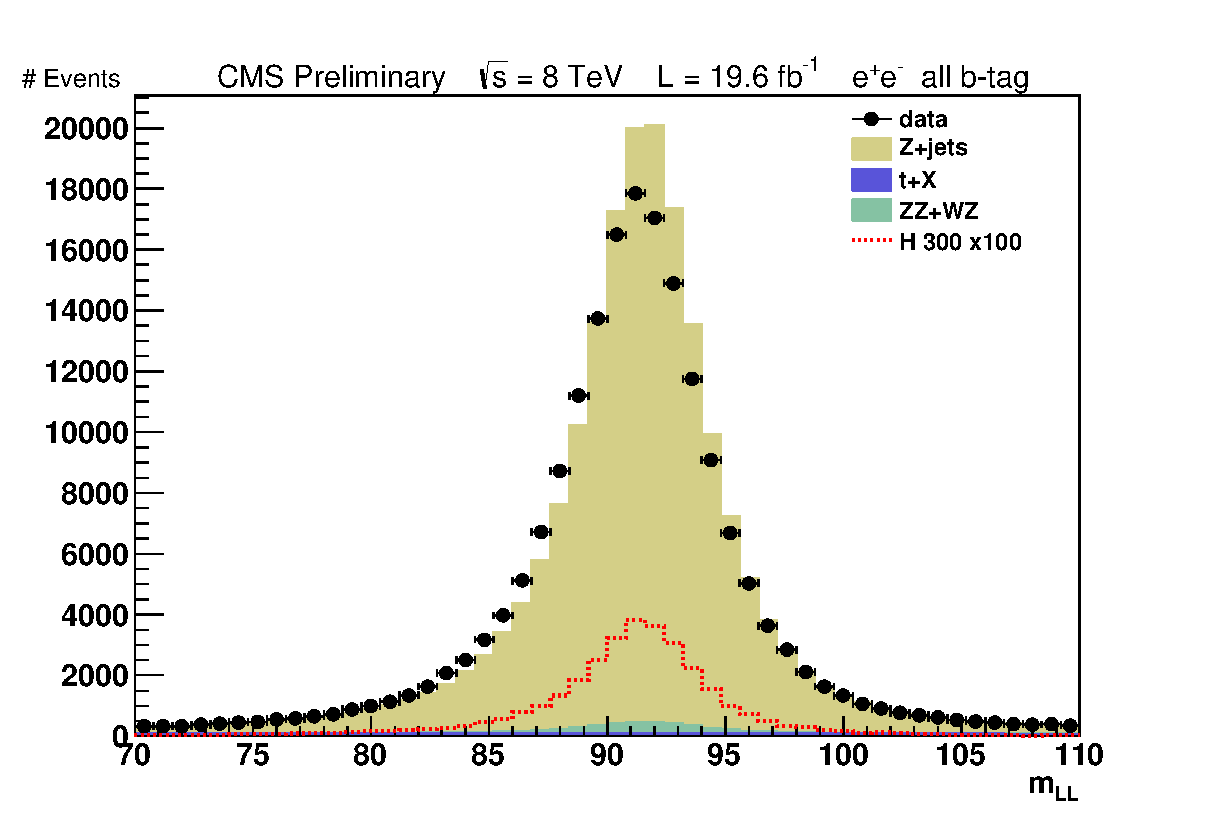
\includegraphics[width=0.47\textwidth]{images/preselection/el/mLL.eps}
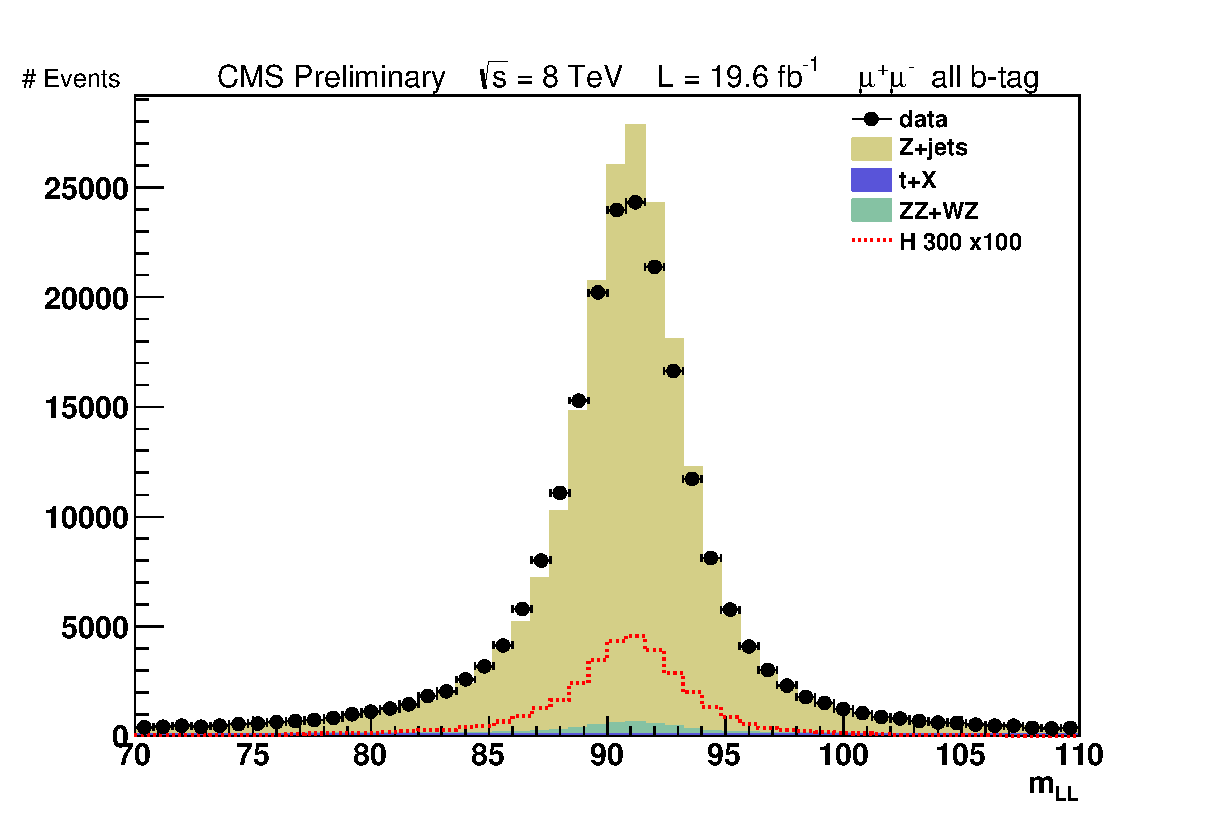
\includegraphics[width=0.47\textwidth]{images/preselection/mu/mLL.eps}\\
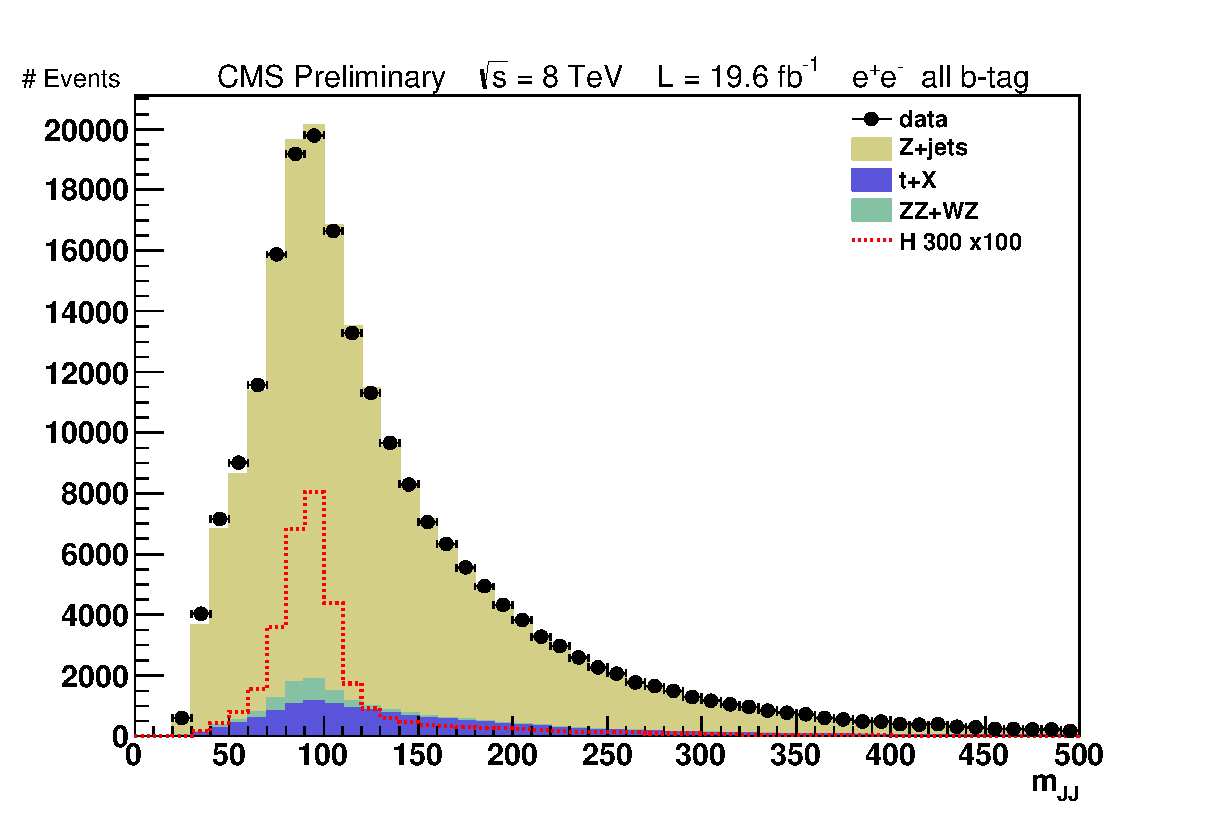
\includegraphics[width=0.47\textwidth]{images/preselection/el/mJJ.eps}
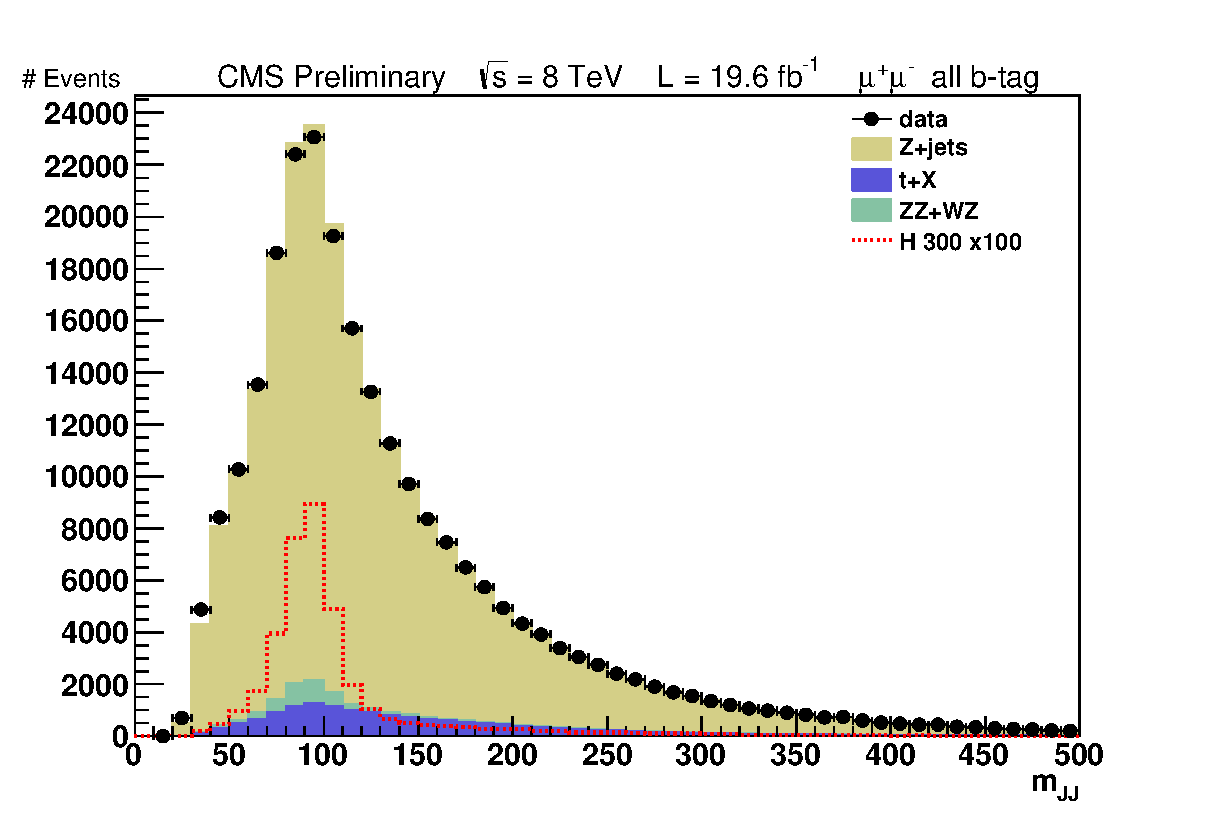
\includegraphics[width=0.47\textwidth]{images/preselection/mu/mJJ.eps}\\
%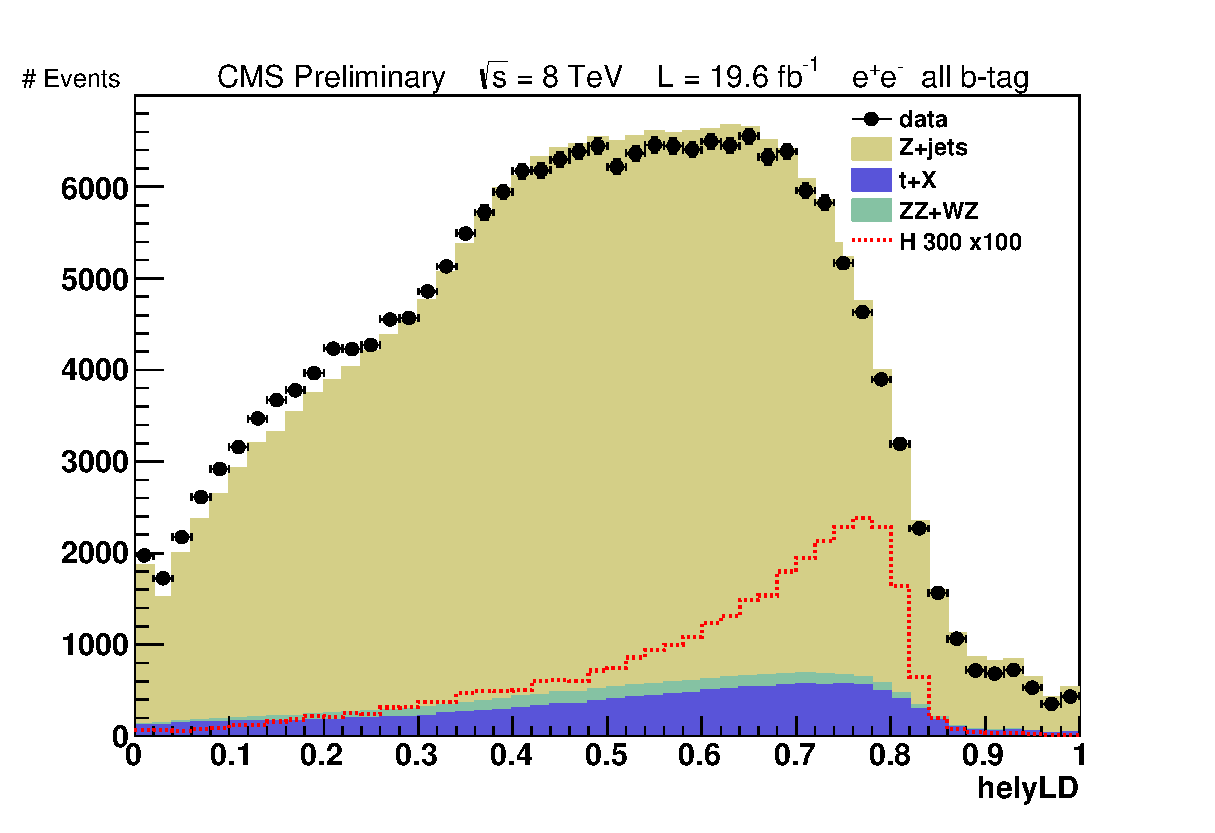
\includegraphics[width=0.4\textwidth]{images/preselection/el/helyLD.eps}
%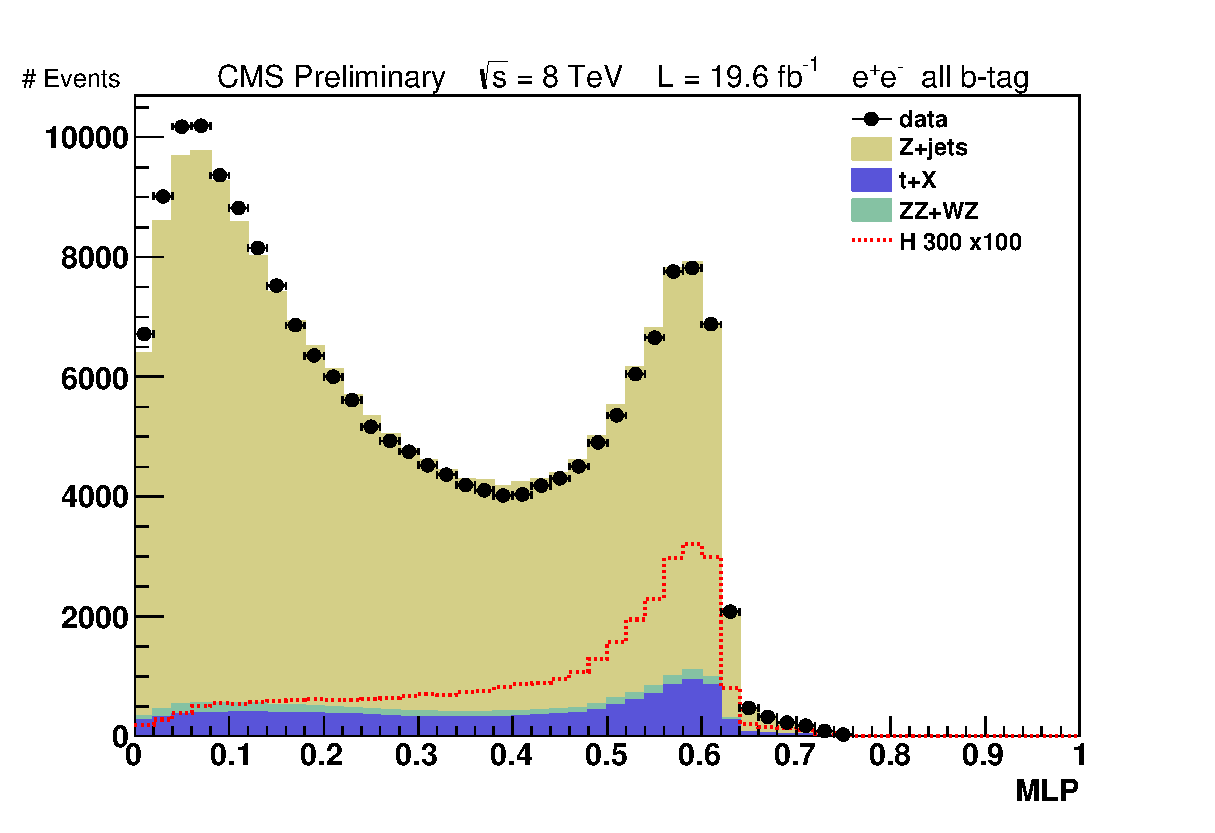
\includegraphics[width=0.4\textwidth]{images/preselection/el/MLP.eps}\\
%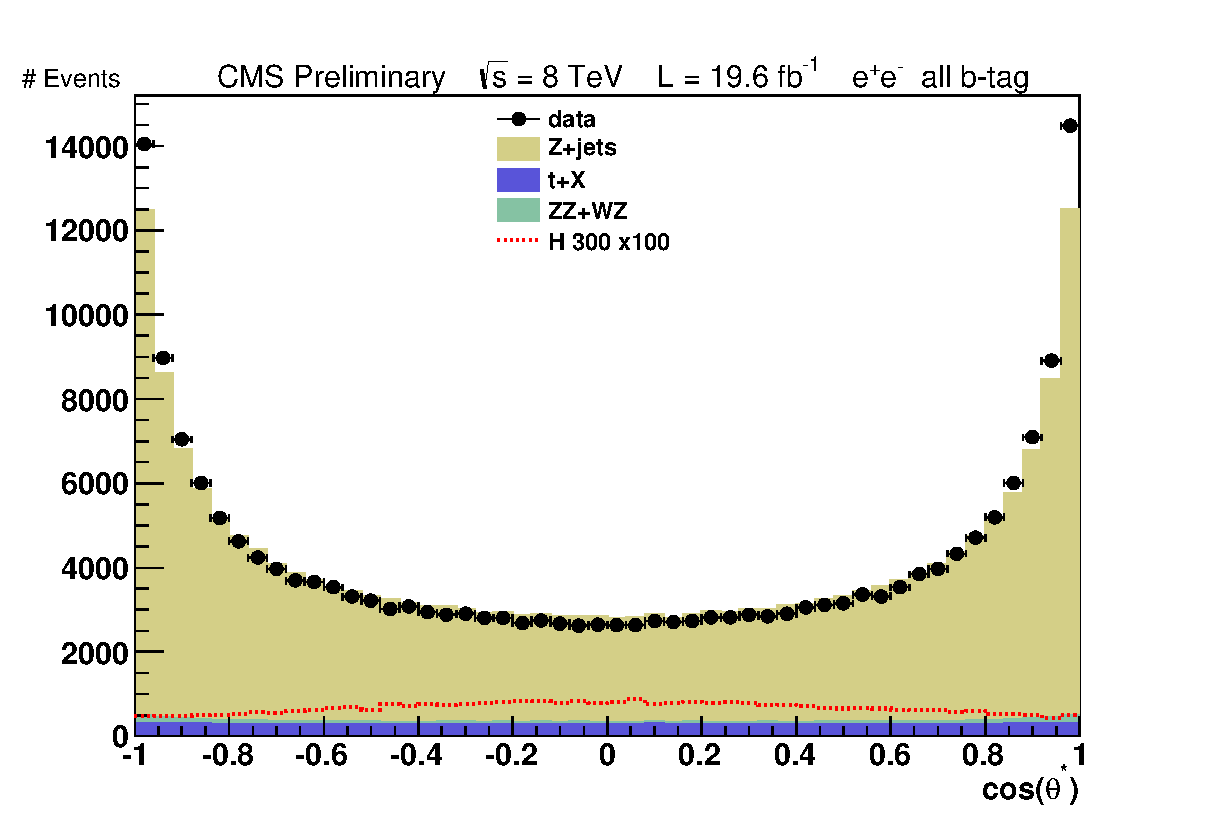
\includegraphics[width=0.4\textwidth]{images/preselection/el/costhetast.eps}
%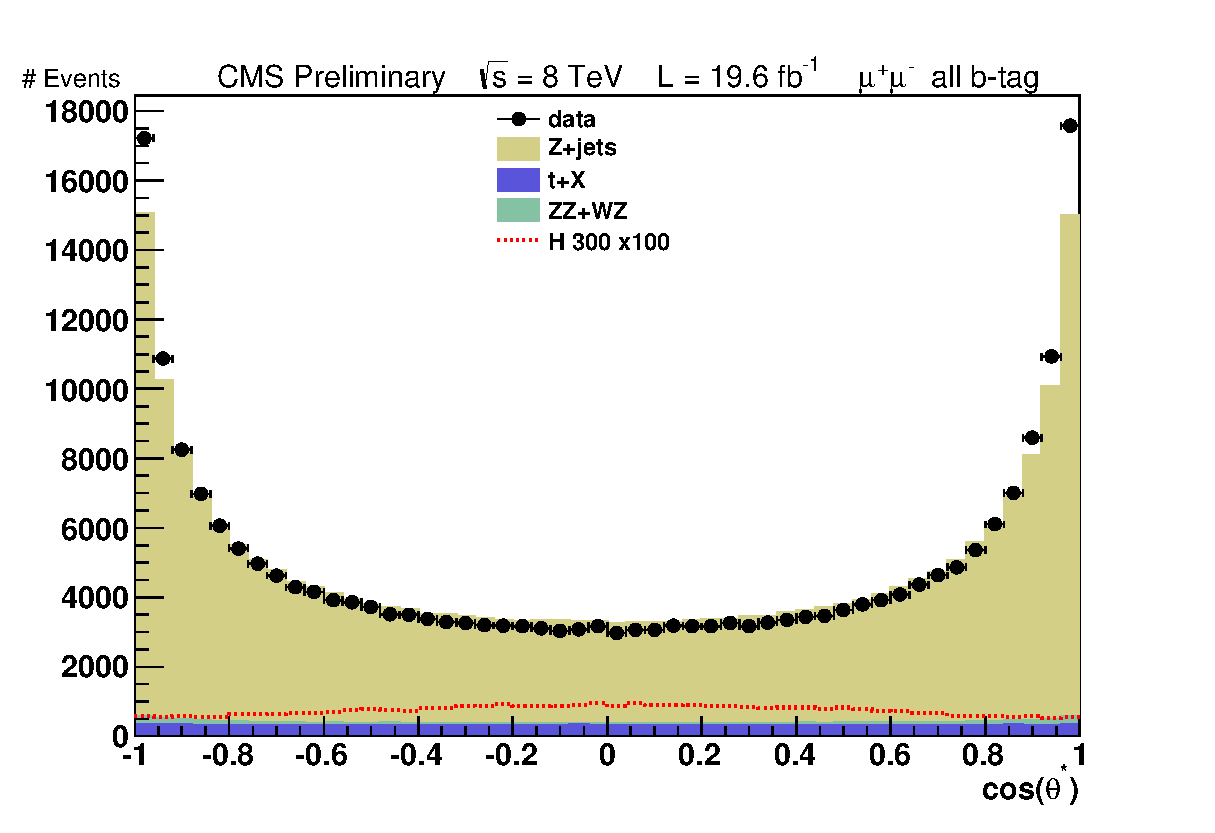
\includegraphics[width=0.4\textwidth]{images/preselection/mu/costhetast.eps}
\end{center}
\end{frame}



%%%%%%%%%%%%%%%%%%%%%%%%%%%%%%%%%%%%%%%%5



\begin{frame}{MLP and HelyLD Data/MC Discrepancy}
\begin{center}
Both the HelyLD and the MLP don't agree in the background like regions between data and MC. This is because $cos(\theta^{*})$ is not well modeled in MC.
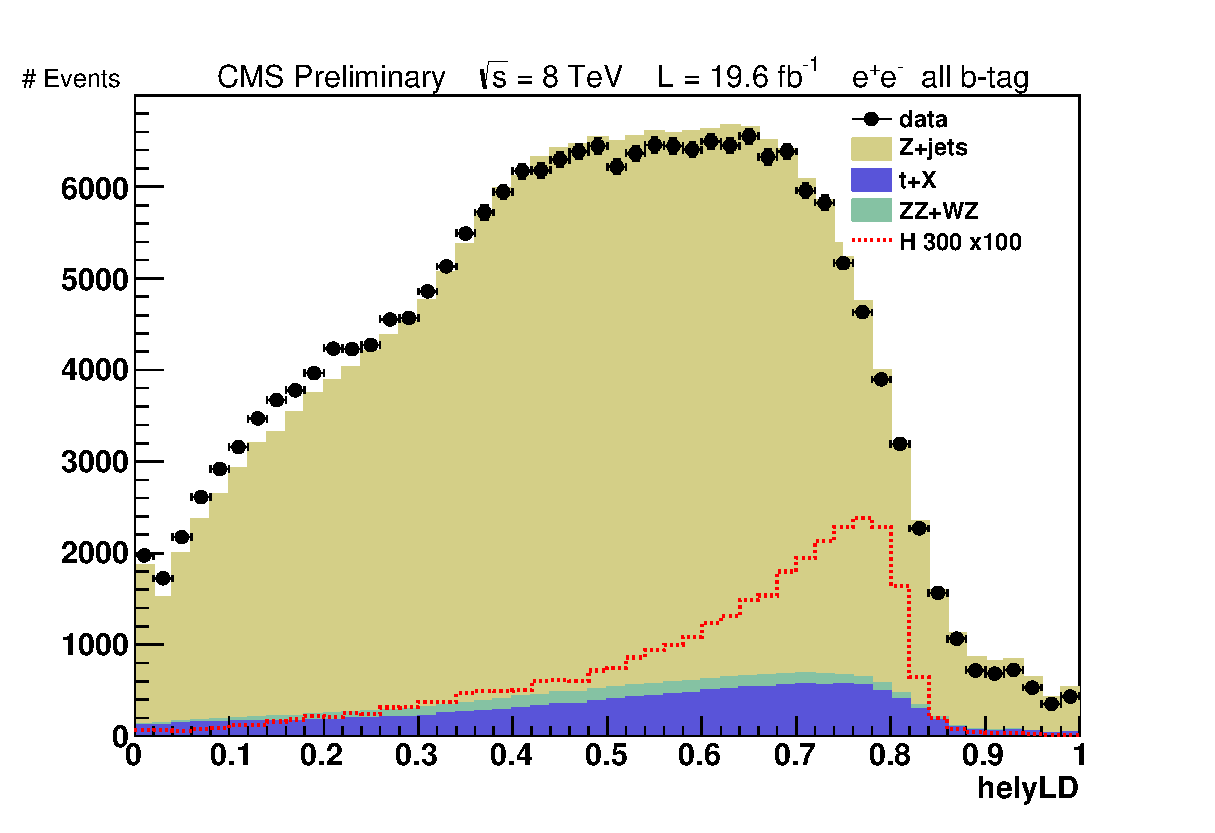
\includegraphics[width=0.4\textwidth]{images/preselection/el/helyLD.eps}
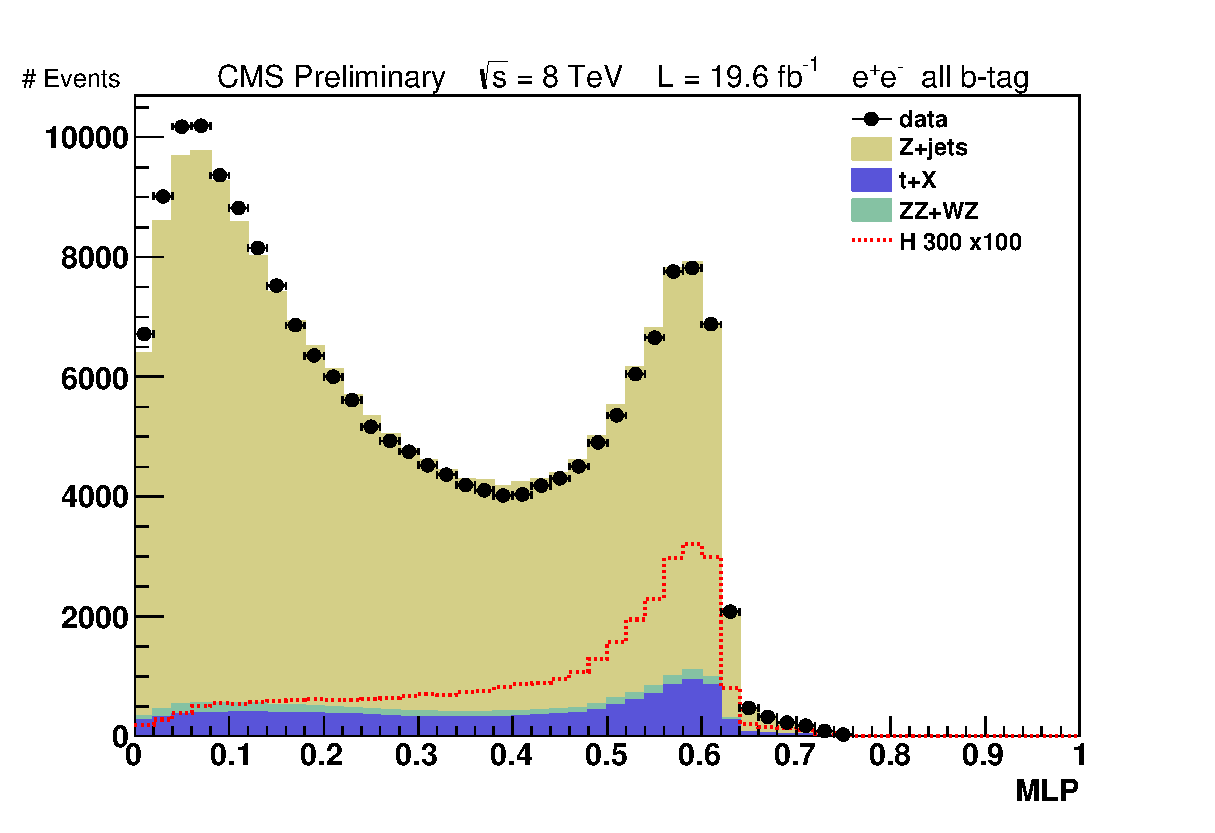
\includegraphics[width=0.4\textwidth]{images/preselection/el/MLP.eps}\\
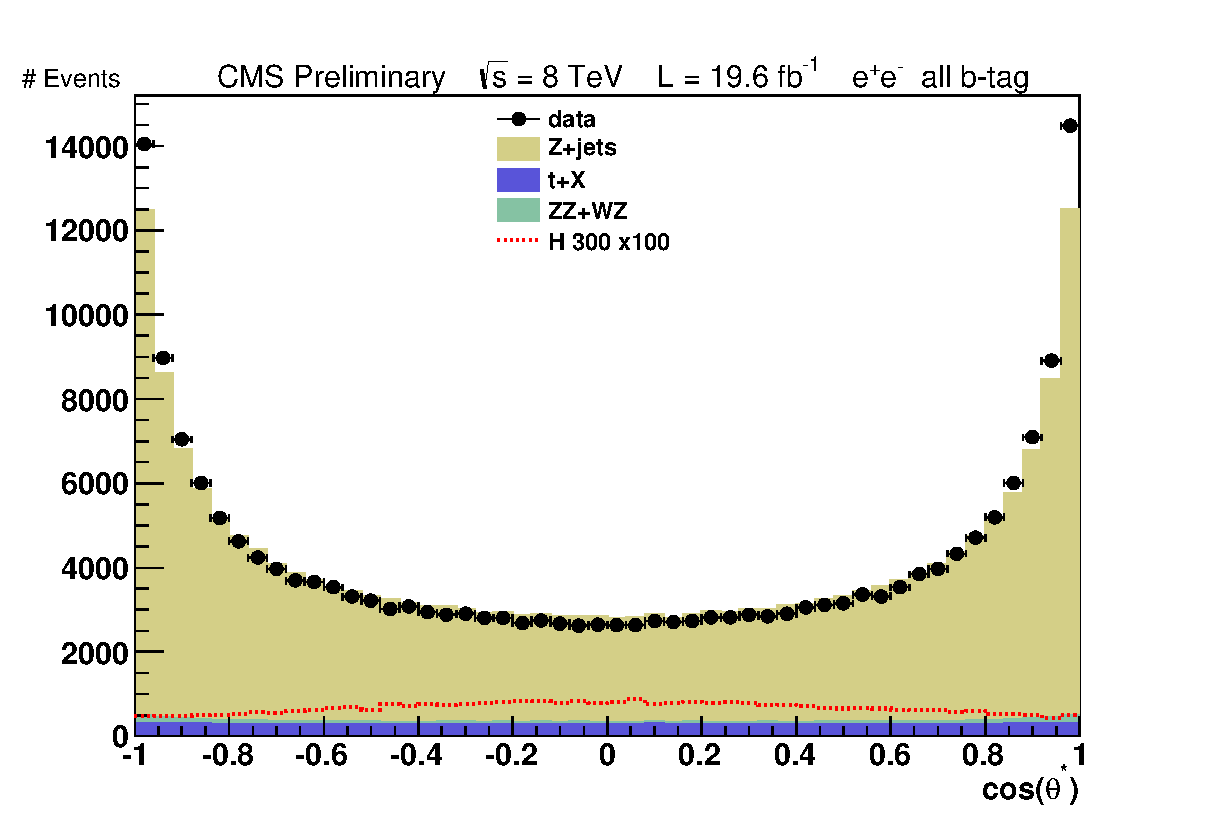
\includegraphics[width=0.4\textwidth]{images/preselection/el/costhetast.eps}
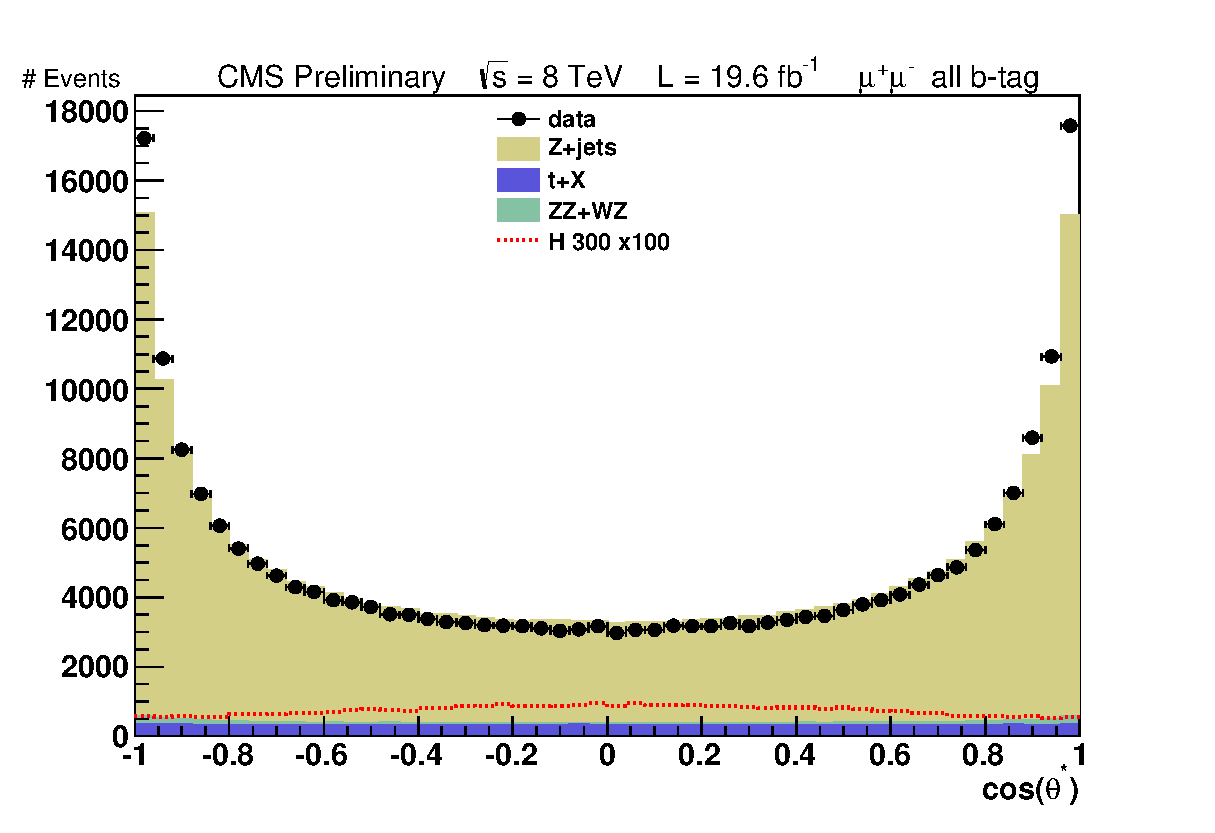
\includegraphics[width=0.4\textwidth]{images/preselection/mu/costhetast.eps}
\end{center}
\end{frame}

\begin{frame}{Solution}
\begin{center}
This is a MC issue that can be fixed by cutting on |$cos(\theta^*)$| > 0.8 or by refitting MC to data.\\
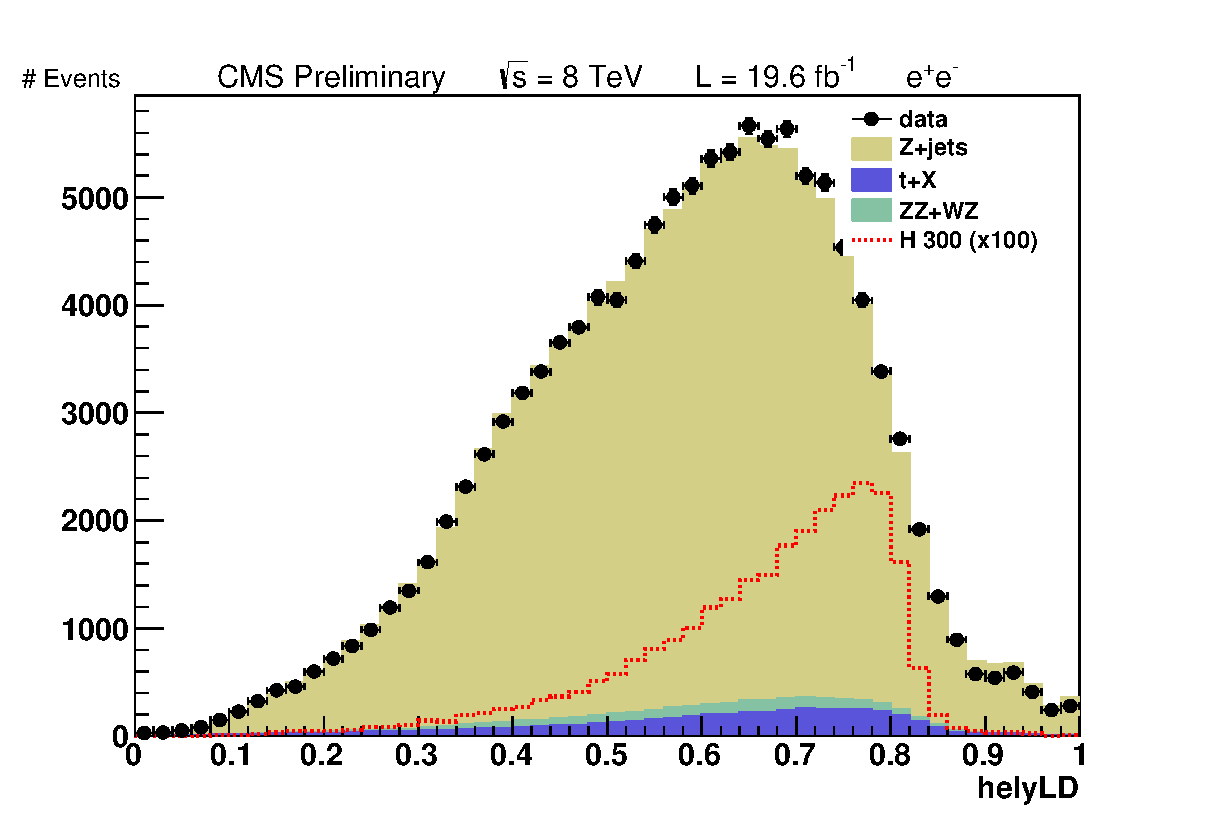
\includegraphics[width=0.4\textwidth]{images/costhetast_cut/el/helyLD.eps}
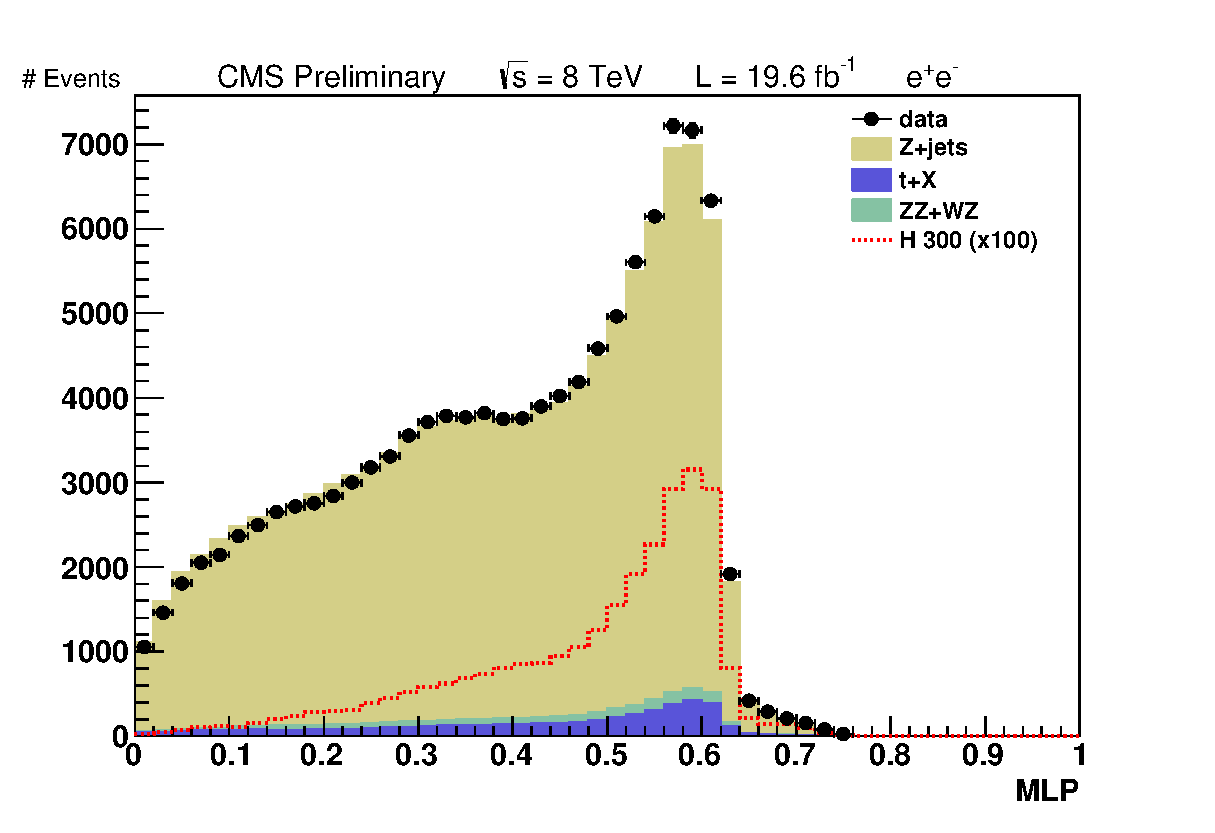
\includegraphics[width=0.4\textwidth]{images/costhetast_cut/el/MLP.eps}\\
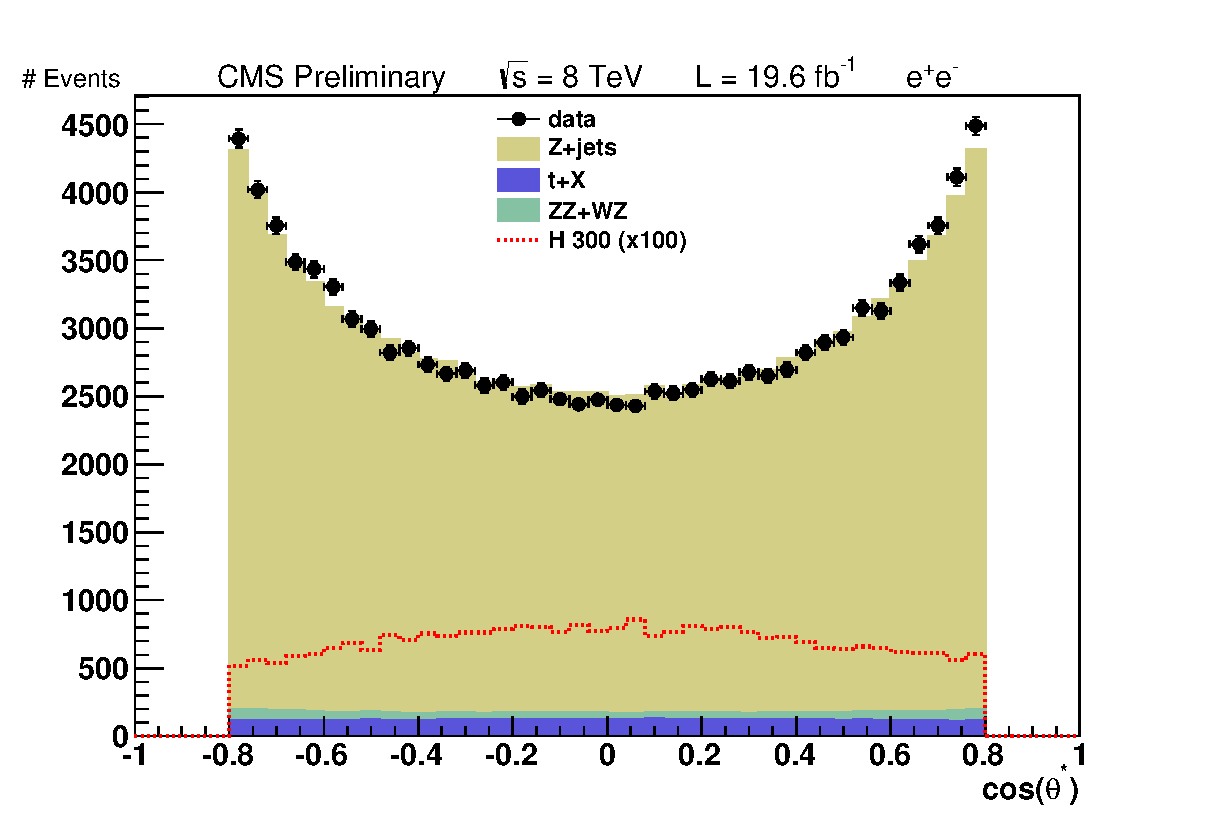
\includegraphics[width=0.4\textwidth]{images/costhetast_cut/el/costhetast.eps}
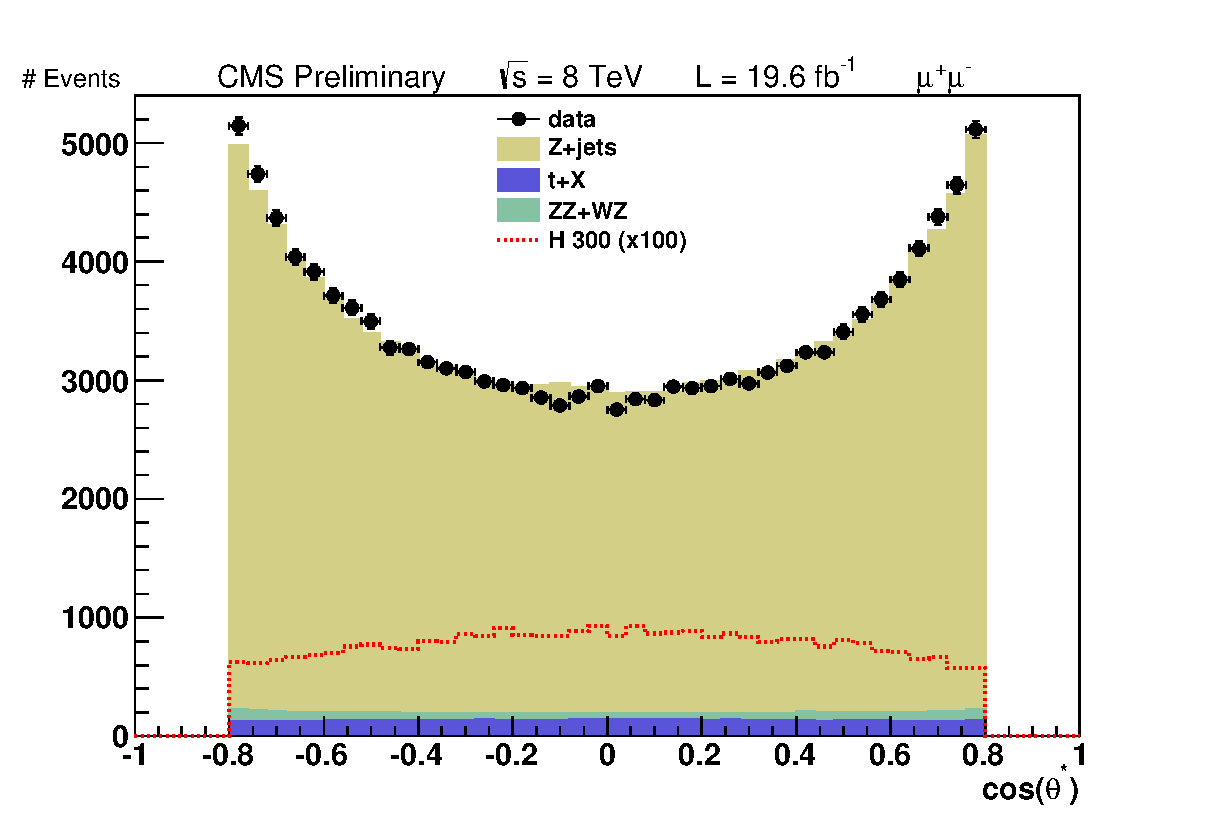
\includegraphics[width=0.4\textwidth]{images/costhetast_cut/mu/costhetast.eps}
\end{center}
\end{frame}




\begin{frame}{2011 Results}
\begin{center}
\scriptsize
Limit on the expected 95$\%$ CL upper limit on the product of the Higgs boson production cross section and the branching fraction of H$\rightarrow$ZZ (black dots.), for the recorded luminosity in 2011 of 4.9 fb$^{-1}$ at 7TeV. Yellow and Green bands represent the 68$\%$ and 95$\%$ ranges of expectation.
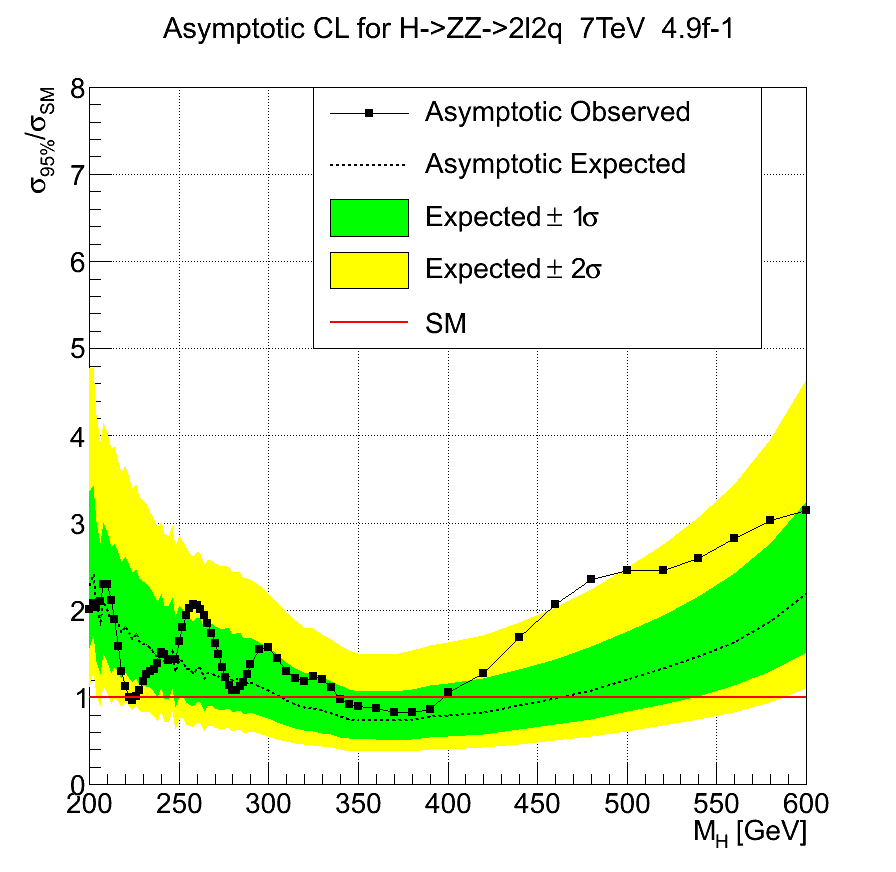
\includegraphics[width=0.5\textwidth]{images/plots/ASCL_7TEV_unblided_new230_new_xsec.png}\\
CMS Collaboration, Search for a Higgs boson in the decay channel $\Htollqq$, JHEP 04 (2012) 036, doi:10.1007/JHEP04(2012)036, arXiv:1202.1416.
\end{center}
\end{frame}



\begin{frame}{Shape vs Cut and Count}
\begin{center}
\scriptsize
%Limit on the expected 95$\%$ CL upper limit on the product of the Higgs boson production cross section and the branching fraction of H$\rightarrow$ZZ (dash line( and observed upper limit (black dots.) Yellow and Green bands represent the 68$\%$ and 95$\%$ ranges of expectation.
\begin{columns}
  \begin{column}{0.5\textwidth}
    \begin{center}
    {\large Shape}\\ 
    \vspace{.2em}
   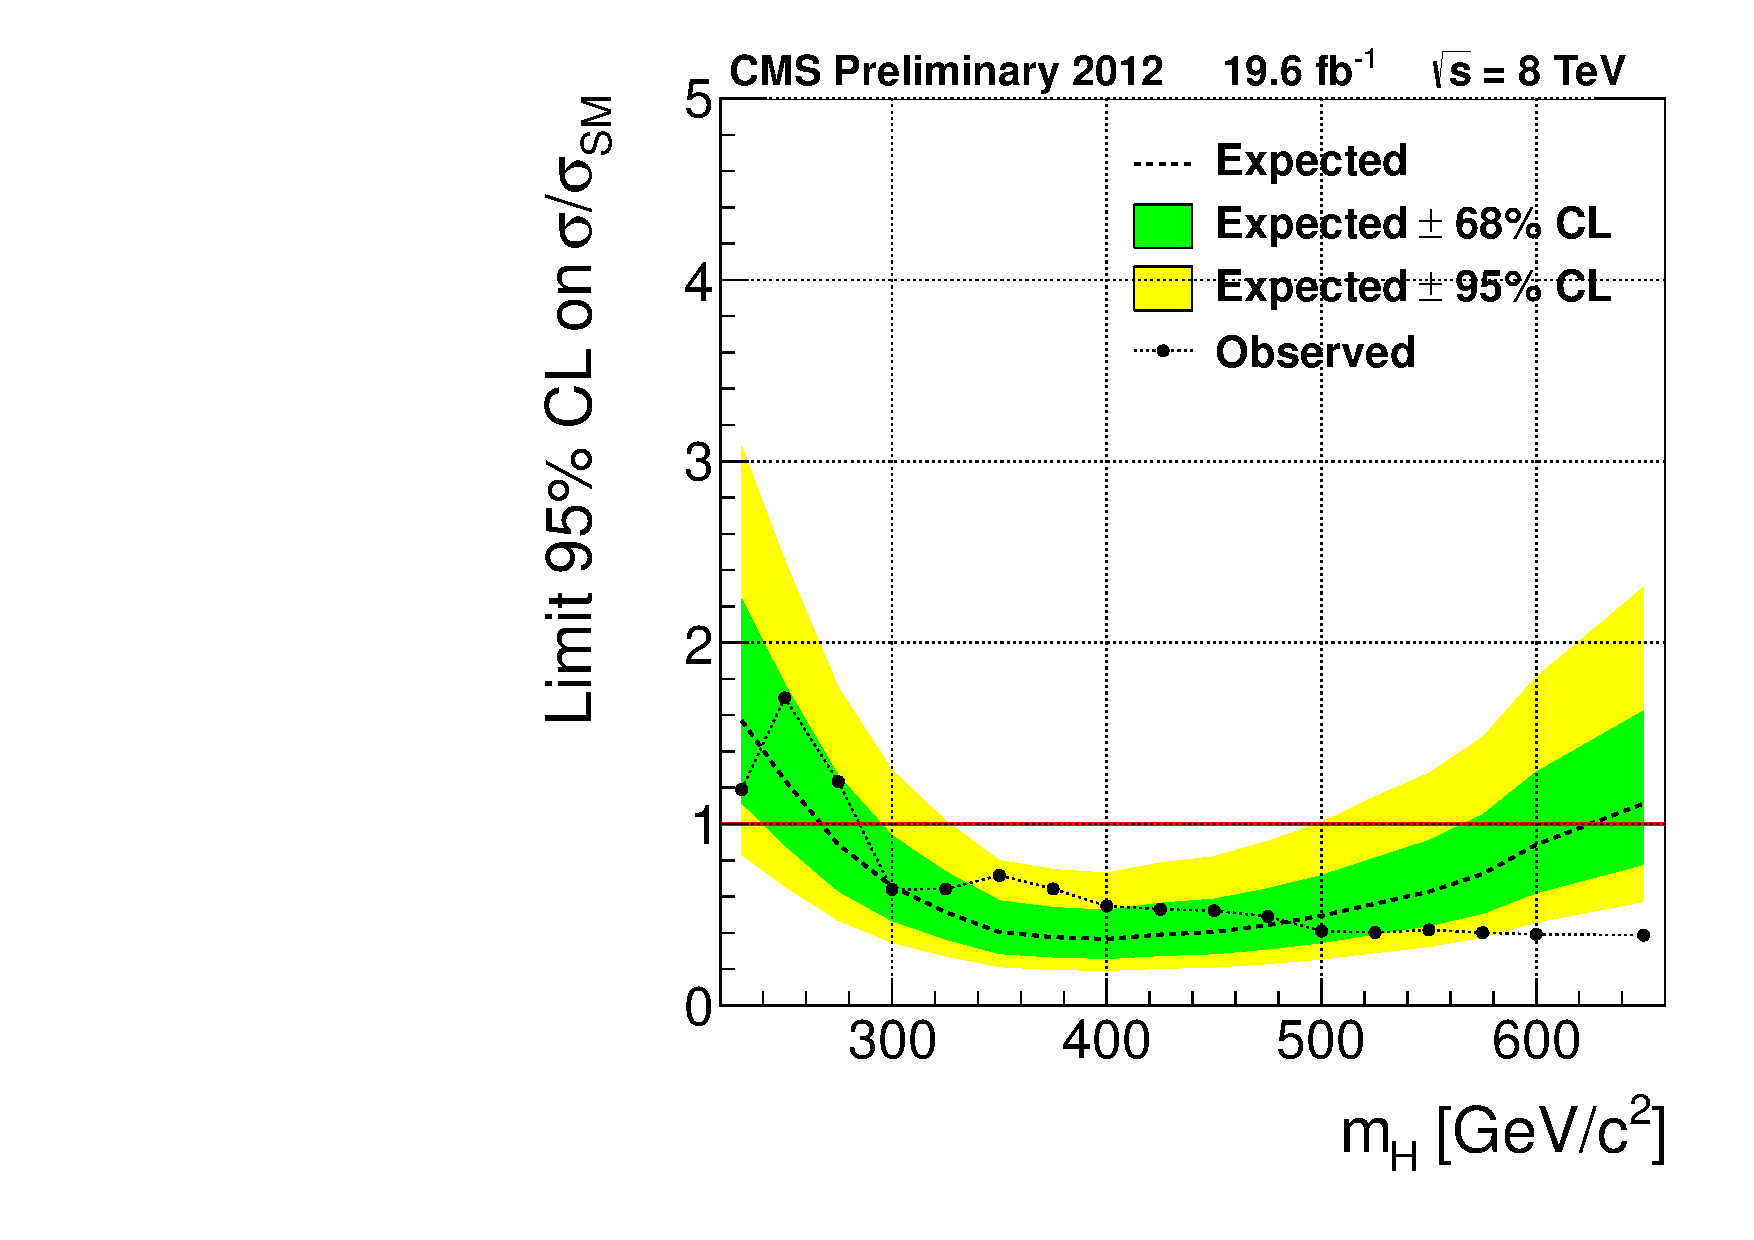
\includegraphics[width=1.\textwidth]{images/8TeV_limit.pdf}
   \end{center}
  \end{column}
  \begin{column}{0.5\textwidth}
    \begin{center}
    {\large Cut and Count}\\
    -6\% m$_H$ +10\%\\
    \vspace{.2em}
    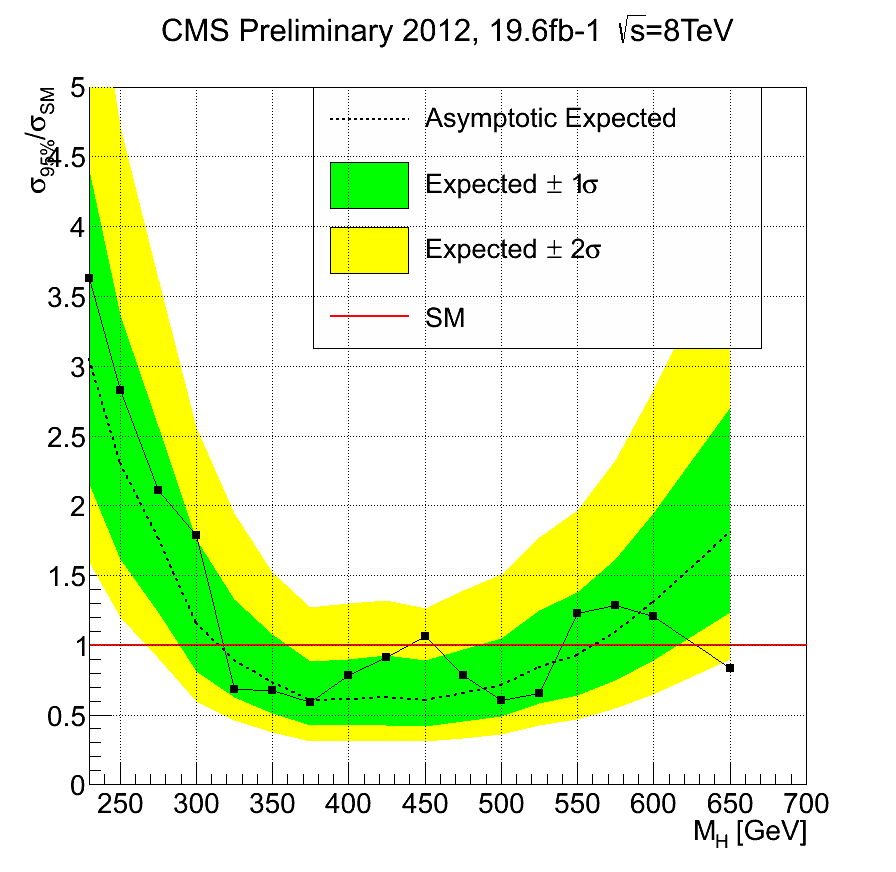
\includegraphics[width=1.\textwidth]{images/cutcount.png}
    \end{center}
  \end{column}
\end{columns}

\end{center}
%\vspace{.2em}
\footnotesize
The shape analysis does about 15\% better than the cut and count, but both give very similar results.  

\end{frame}



%\begin{frame}{Pile-up Rejection}
%\begin{center}
% $\beta$ is the sum of transverse momenta of all charged particles in the jet coming from the primary vertex, normalized to the total sum of transverse momenta of all charged particles in the jet.
% \begin{itemize}
%  \item
%    Using $\beta$ variable to remove candidates with PU-like jets 
%  \item
%    Cutting on $\beta \geq$~0.2
%  \end{itemize}

%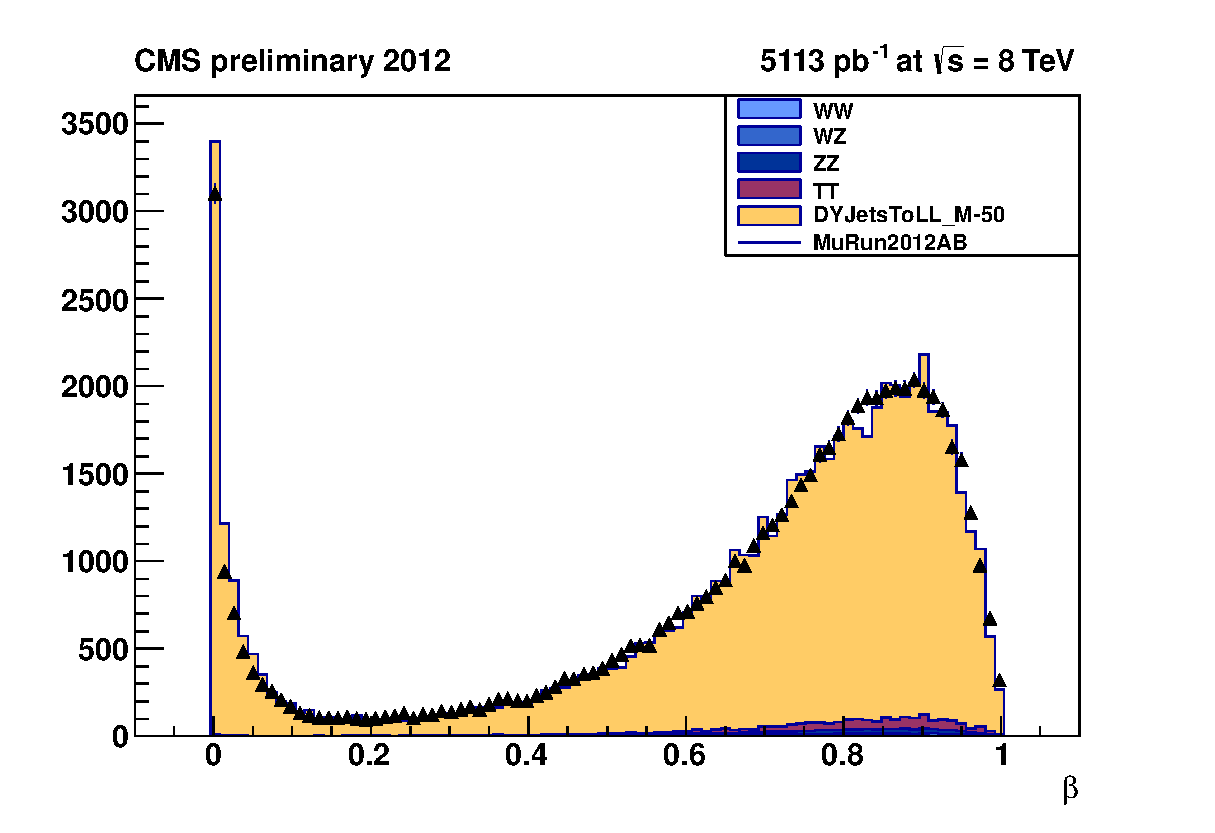
\includegraphics[width=0.59\textwidth]{images/beta_MuRun2012.eps}
%\end{center}
%\end{frame}

%\begin{frame}{$\dfrac{Signal}{\sqrt{Signal + Background}}$}
%\begin{center}
%400GeV Training
%  \begin{tabular}{ | c | c | c | c | c | c | c |}
%    \hline
%    & \multicolumn{3}{|c|}{Electron} & \multicolumn{3}{|c|}{Muon}\\ \hline
%    Sample  & zero& one  & two  & zero & one  & two  \\ \hline \hline
%GG600 & 0.215 & 0.224 & 0.309 & 0.232 & 0.210 & 0.345\\ \hline
%GG700 & 0.086 & 0.089 & 0.121 & 0.088 & 0.083 & 0.134\\ \hline
%GG800 & 0.035 & 0.036 & 0.052 & 0.036 & 0.033 & 0.057\\ \hline
%GG900 & 0.016 & 0.016 & 0.023 & 0.016 & 0.015 & 0.025\\ \hline
%GG1000 & 0.009 & 0.009 & 0.012 & 0.009 & 0.008 & 0.013\\ \hline
%\end{tabular}
%\\
%800GeV Training
%\begin{tabular}{ | c | c | c | c | c | c | c |}
%    \hline
%    & \multicolumn{3}{|c|}{Electron} & \multicolumn{3}{|c|}{Muon}\\ \hline
%    Sample  & zero& one  & two  & zero & one  & two  \\ \hline \hline
%GG600 & 0.204 & 0.223 & 0.297 & 0.225 & 0.198 & 0.344\\ \hline
%GG700 & 0.084 & 0.091 & 0.118 & 0.088 & 0.082 & 0.140\\ \hline
%GG800 & 0.035 & 0.039 & 0.053 & 0.038 & 0.034 & 0.061\\ \hline
%GG900 & 0.017 & 0.018 & 0.023 & 0.017 & 0.016 & 0.027\\ \hline
%GG1000 & 0.009 & 0.009 & 0.012 & 0.009 & 0.009 & 0.014\\ \hline
%\end{tabular}\end{center}
%\end{frame}

%\begin{frame}{Difference in $\dfrac{Signal}{\sqrt{Signal + Background}}$ 400 vs 800}
%\begin{center}
%  \begin{tabular}{ | c | c | c | c | c | c | c |}
%    \hline
%    & \multicolumn{3}{|c|}{Electron} & \multicolumn{3}{|c|}{Muon}\\ \hline
%    Sample  & zero& one  & two  & zero & one  & two  \\ \hline \hline
%
%GG600 & 4.93\% & 0.18\% & 4.17\% & 2.98\% & 5.49\% & 0.33\% \\ \hline
%GG700 & 1.72\% & -2.75\% & 2.58\% & 0.36\% & 1.57\% & -3.91\% \\ \hline
%GG800 & -1.71\% & -7.89\% & -2.51\% & -4.42\% & -2.47\% & -7.02\% \\ \hline
%GG900 & -2.87\% & -8.16\% & 0.30\% & -5.16\% & -4.40\% & -8.41\% \\ \hline
%GG1000 & -2.62\% & -8.38\% & -1.75\% & -4.26\% & -2.13\% & -10.91\% \\ \hline
%
%\end{tabular}
%\end{center}
%
%\end{frame}
